\documentclass{eceday}

\graphicspath{{./Images/}}
\addbibresource{../References.bib}

\title[Chipyard]{Chipyard: A RISC-V Development Framework}
\subtitle{ECE Day 2021}
\author{Alexander Lukens \and Karl Hallsby}
\institute{Illinois Institute of Technology}
\date{\DTMdisplaydate{2021}{4}{9}{-1}}

\begin{document}

\nocite{chipyard}

\begin{frame}
  \titlepage{}
\end{frame}

\section{About Us}\label{sec:About_Us}
\begin{frame}
  \frametitle{\nameref{sec:About_Us}}
  \begin{figure}[h!tbp]
    \centering
    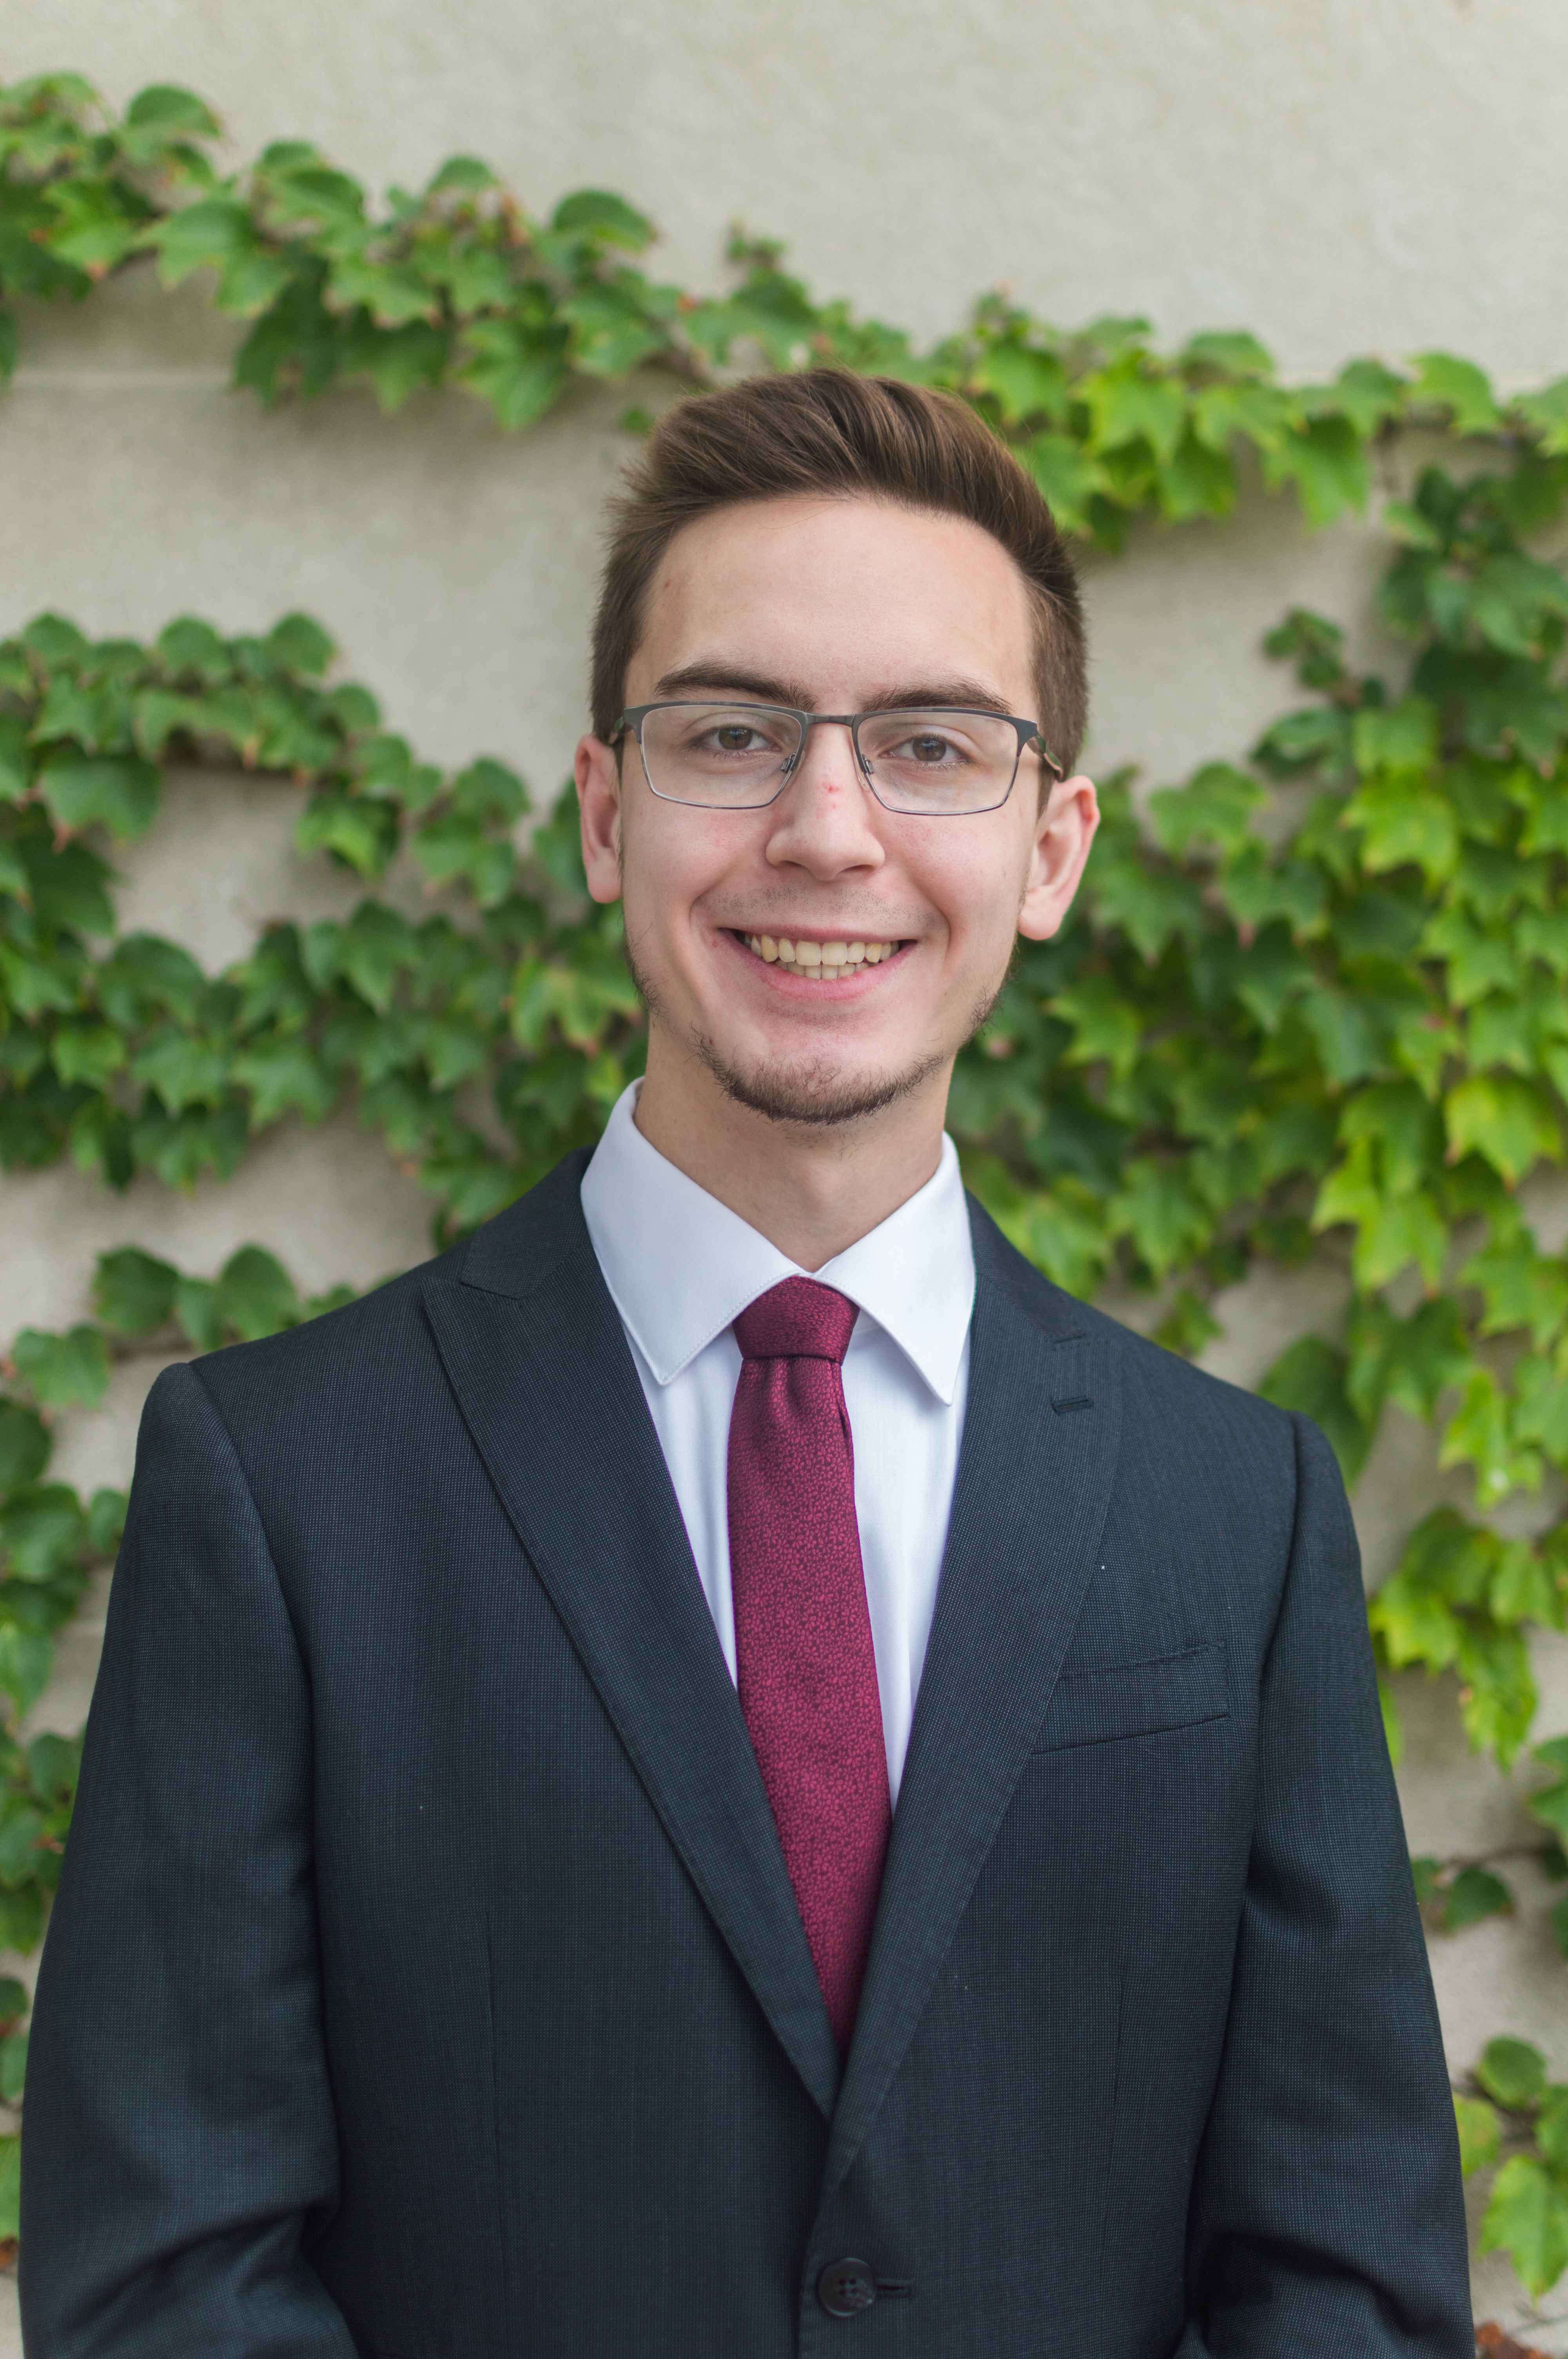
\includegraphics[width=0.25\linewidth]{./Lukens_Alex.jpg}
    \caption*{Alexander Lukens}
    \label{fig:Alex_Lukens}
  \end{figure}
  \begin{figure}[h!tbp]
    \centering
    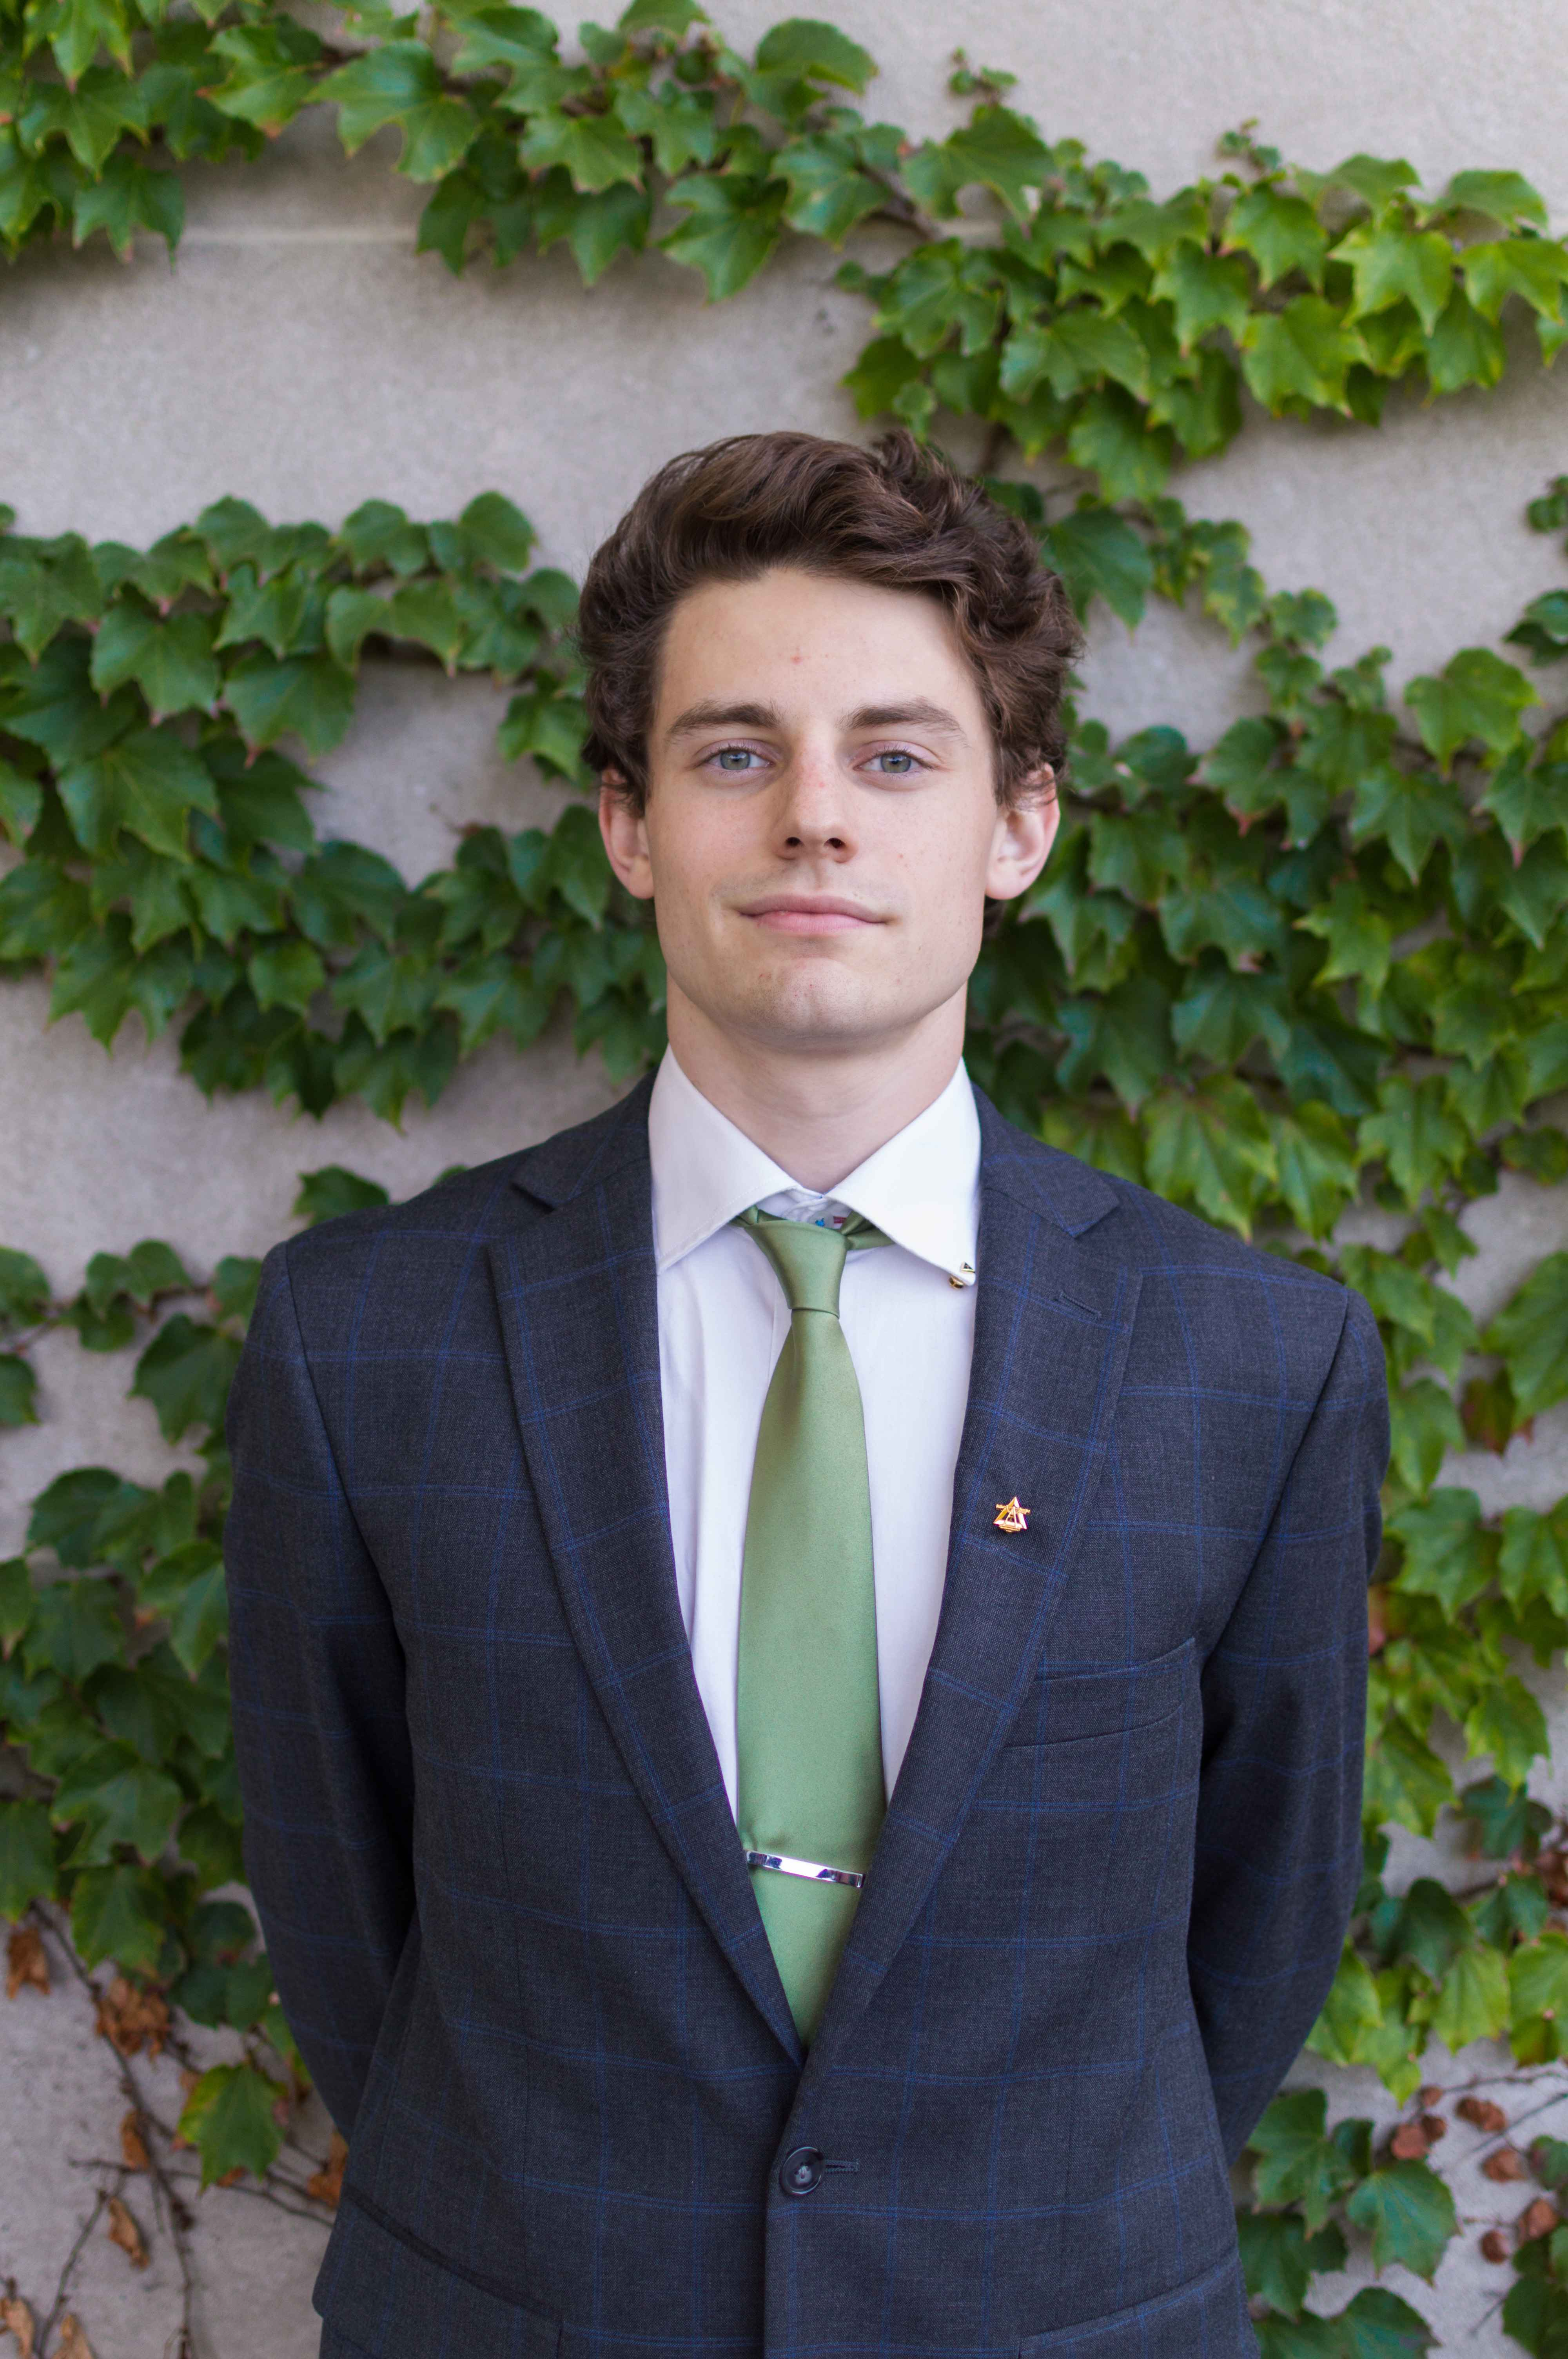
\includegraphics[width=0.25\textwidth]{./Hallsby_Karl.jpg}
    \caption*{Karl Hallsby}
    \label{fig:Karl_Hallsby}
  \end{figure}
\end{frame}

\section{What is RISC-V?}\label{sec:What_is_RISC-V}
\begin{frame}
  \frametitle{\nameref{sec:What_is_RISC-V}}
\end{frame}

\section{What is Chipyard?}\label{sec:What_is_Chipyard}
% Image of silicon they've taped out using Chipyard and its associated tools
\begin{frame}
  \frametitle{\nameref{sec:What_is_Chipyard}}
\end{frame}

\end{frame}

\section{What We Learned}\label{sec:What_We_Learned}
\begin{frame}
  \frametitle{What We Learned}
\end{frame}

\section{Next Steps}\label{sec:Next_Steps}
\begin{frame}
  \frametitle{Next Steps}
\end{frame}

\begin{frame}
  \frametitle{References}

  \printbibliography[heading=bibintoc]{}
\end{frame}

\end{document}

%%% Local Variables:
%%% mode: latex
%%% TeX-master: t
%%% End:
